\chapter{预备知识}
本章将要介绍的预备知识包括饱和流量、饱和流率、信号相位以及绿“波带灯”。接着介绍K-Means均值聚类算法和二次规划算法。
%本章将介绍文章中所涉及的预备知识,包括饱和流量和饱和流率、信号相位和“绿波带”等交通工程相关知识,还包括了。
\section{交通工程相关理论}

\subsection{饱和流量与饱和流率}
饱和流量,指的是在单元时间内车辆经过十字路口停车线的最大流量\cite{wuzhen2008}。饱和流率指当信号灯转为绿灯状态后,放行车流率逐渐达到稳定值,此时的放行车流率即为饱和流率\cite{liuyi2010}。

%车辆通过交叉口的放行车流率逐渐达到稳定值,这个稳定的值即为饱和流率\cite{liuyi2010}。在车流率达到饱和车流率后,尚未越过停车线的车流流量将继续保持饱和车流量,直到绿灯结束或是车辆全部通行完毕。

%饱和流量指的是单位时间内车辆通过交叉路口停车线的最大流量,即路口的排队车辆加速到正常行驶速度时,单位时间内通过路口停车线的稳定车流量\cite{wuzhen2008}。饱和流率指当信号灯变为绿灯时,车辆通过交叉口的放行车流率逐渐达到稳定值,这个稳定的值即为饱和流率\cite{liuyi2010}。在车流率达到饱和车流率后,尚未越过停车线的车流流量将继续保持饱和车流量,直到绿灯结束通行时间截止或是车辆全部通行完毕。

%当交通信号灯转变为绿灯显示时,原先等候在停车线后面的车流便开始向前运动,车辆鱼贯地越过停车线,其放行车流率,由零很快增至一个稳定的数值,即饱和流率\cite{liuyi2010}。此后,越过停车线的后续车流流量将继续保持与饱和流量相等,直到停车线后面原先积存的车辆全部放行完毕,或者虽未放完,但放行时间已经截止。

%影响道路饱和流量大小的道路条件主要有车道的宽度、车道的坡度,影响道路饱和流量大小的车流状况主要有大车混入率、转弯车流的比率、车道的功能\cite{wuzhen2009},影响道路饱和流量大小的配时方案主要指信号相位的设置情况\cite{likeping2007}。

%饱和流量值应尽量通过现场实地观测求得,但在某些情况下,尤其是在设计一个新的交叉口时,由于无法使用实测的方法求得饱和流量值,此时可以使用一些公式或图表来近似求取道路的饱和流量值\cite{shaochangqiao2011,lihongqiang}。常用的计算方法有韦伯斯特法\cite{wangjiawen2021}、曲线法\cite{1988Using}、折算系数法、停车线法、冲突点法\cite{xuliqun2001}等。
影响车道饱和流量的各种因素大致包括路面条件、车流情况以及配时方法三种。路面条件主要和车道的宽窄、坡度相关;车流状况主要与大车混入率、转弯车流比和车道预设功能有关\cite{wuzhen2009};配时方案主要与道路交叉口信号相位设置有关\cite{likeping2007}。针对已达到使用状况并有实际车流量的路口,通过在路口处实际观察可以计算出饱和流量值。但是在某些无法实地观测的场景下,例如在全新道路交叉口的设计阶段,无法通过实地观测统计出饱和流量值,此时需要选用合适的理论方法近似估算道路的饱和流量值\cite{shaochangqiao2011}。常用的估算饱和流量值的算法有曲线法\cite{1988Using}、冲突点法\cite{xuliqun2001}、韦伯斯特法\cite{wangjiawen2021}等。

\subsection{信号相位}
通过给不同方向的交通流按时间片分配通行权的方式,可以有效避免以二维交叉口为主的在空间上相交的道路存在的各向交通流之间的冲突。在交通信号系统中,不同国家对交通信号相位的基本概念定义不尽相同。美国的《通行能力手册》\cite{2000Highway}将相位定义为分配给在一个或多个时间间隔内,获得通行权的任何交通流组合的部分信号周期。联邦公路管理局将信号相位定义为分配给独立或组合交通流循环中的绿灯通行、黄灯改变和红灯等待\cite{2003Manual}。在中国,《交通管理与控制》\cite{yangpeikun2003}认为,在信号控制十字路口,每一个信号状态,即交叉口各个方向上所呈现的各种灯色组合,形成了一种信号相位。根据国家标准\cite{GB_T_31418}规定:信号相位是同时获得通行权的一股或多股交通流对应信号组的显示状态。

%根据中国国家标准GB/T31418-2015[54]中道路信息系统术语二点三.六中的规定:道路信息相位关系是指同一时间拥有车辆通行权的一股或多股道路交通流及其相应信息组的表示状况。

%将月相界定为分派给在一个或多个小时间隔内,以获得通行性的所有交通流组合的部分信号周期。美国联邦高速公路局(FHWA)出版的《统一交通控制设施手册》[52]中将信号月相界定为,分配于单独或混合交通流循环中的绿灯通行时间、黄灯改变和红灯等待。

%在空间上无法实现分离的地方(主要是在平面交叉口上),为了避免不同方向交通流之间的相互冲突,可以通过在时间上给各个方向交通流分配相应的通行权。在交通信号系统中,不同国家对交通信号相位的基本概念定义并不完全相同。在美国《通行能力手册》(Highway Capacity Manual,简称HCM)\cite{2000Highway}将相位定义为分配给在一个或多个时间间隔内,获得通行权的任何交通流组合的部分信号周期。联邦公路管理局(FHWA)出版的《统一交通控制设施手册》(Manual on Uniform Traffic Control Devices,简称MUTCD)\cite{2003Manual}将信号相位定义为分配给独立或组合交通流循环中的绿灯通行、黄灯改变和红灯等待。在中国《交通管理与控制》\cite{yangpeikun2003}中认为,在信号控制交叉口,每一种控制状态(一种通行权),即对各进口道不同方向所显示的不同灯色的组合,成为一个信号相位。根据标准GB/T 31418-2015中道路交通信号控制系统术语2.3.6中规定:信号相位是同时获得通行权的一股或多股交通流对应信号组的显示状态\cite{GB_T_31418}。


%信号相位是根据交叉口通行权在一个周期内的更迭来划分的。一个交通信号控制方案在一个周期内有几个信号相位,则称该信号控制方案为几相位的信号控制。如果相位数设计得太少,则不能有效地分配好路口通行权,路口容易出现交通混乱,交通安全性下降;如果相位数设计得太多,虽然路口的交通次序与安全性得到了改善,但由于相位之间进行转换时都会损失一部分旅行时间,过多的相位数会导致路口的通行能力下降,延长司机在路口的等待时间\cite{shenjiajun2014}。目前我国普遍采用的是两相位到四相位控制\cite{shuaibing}。

%如果相位数设计得太少,则不能有效地分配好路口通行权,路口容易出现交通混乱,交通安全性下降;如果相位数设计得太多,虽然路口的交通次序与安全性得到了改善,但由于相位之间进行转换时都会损失一部分旅行时间,过多的相位数会导致路口的通行能力下降,延长司机在路口的等待时间\cite{shenjiajun2014}。目前我国普遍采用的是两相位到四相位控制\cite{shuaibing}。

一个周期内的相位数量太少,则道路交通上容易发生混乱,而如果相位数量太多,道路上交通次序的可靠性获得了提高,但是相位切换的时间变多,反而降低了通行能力\cite{shenjiajun2014}。目前我国普遍采用的是两相位到四相位控制\cite{shuaibing}。以我国最常见的十字路口为例(如图\ref{fig:intersection_sample}),十字路口分为东、西、南、北四个方向,每个方向都有三个入口车道,分别为左转、直行和右转。其间最左边的车辆道为左转,中间的车辆道为直行,最右边的车辆道则为右拐,因此每个路口需要${3\times4=12}$个交通信号灯。


\begin{figure}[H]
	\centering
	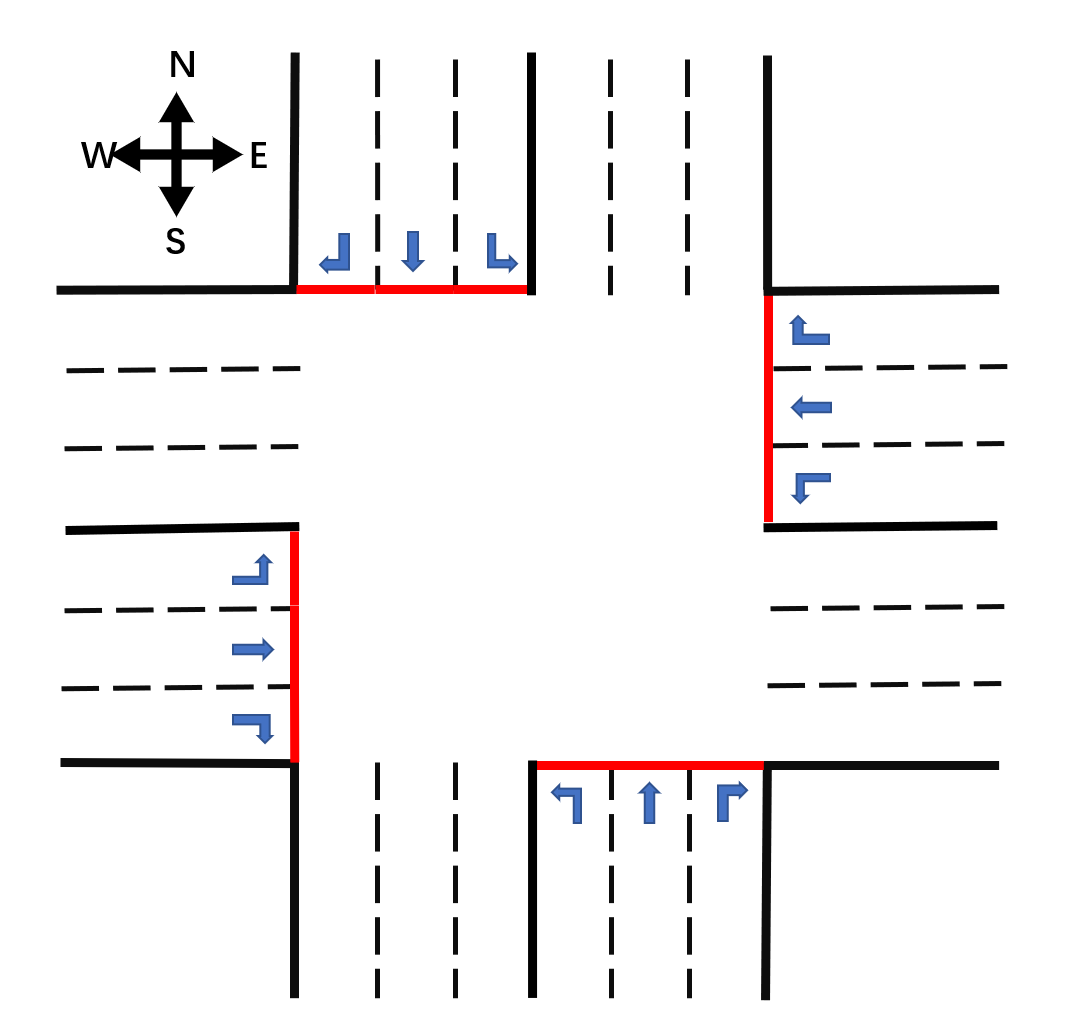
\includegraphics[width=0.6\textwidth]{figures/intersection_sample.png}
	\caption{十字交叉路口样例}
	\label{fig:intersection_sample}
\end{figure}
%交叉路口各入口车道不同方向交通灯所显示的红黄绿三种灯色组合构成不同的信号相位。该十字路口存在四种互不冲突的信号相位,分别是:(1)东西方向直行及右转;(2)东西方向左转;(3)南北方向直行及右转;(4)南北方向左转。十字路口交通灯信号相位如图\ref{fig:intersection_phase}所示。

%T型交叉路口通常使用两相位组成信号相位,分别是:(1)东西方向直行及右转;(2)南北方向左转及右转。具体信号相位图如\ref{fig:T_intersection_phase}所示。

交叉路口各入口车道不同方向交通灯所显示的红黄绿三种灯色组合构成不同的信号相位。该十字路口存在四种互不冲突的信号相位,分别是:(1)东西方向直行及右转;(2)东西方向左转;(3)南北方向直行及右转;(4)南北方向左转。十字路口交通灯信号相位如图\ref{fig:intersection_phase}所示。
\begin{figure}[H]
	\centering
	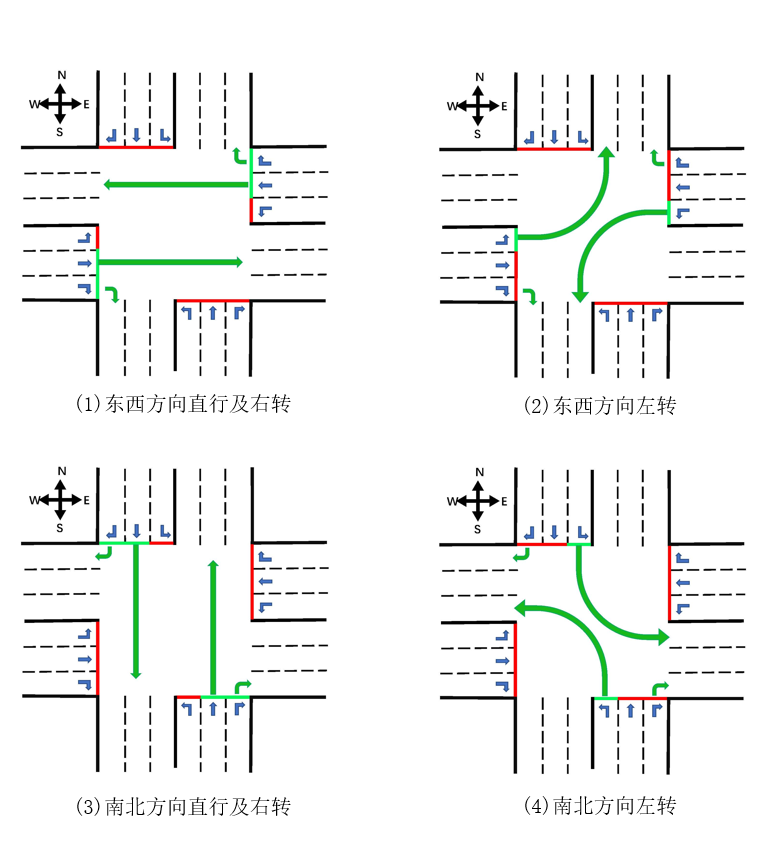
\includegraphics[width=\textwidth]{figures/intersection_phase.png}
	\caption{十字路口交通灯信号相位}
	\label{fig:intersection_phase}
\end{figure}

%T型交叉路口通常使用两相位组成信号相位,分别是:(1)东西方向直行及右转;(2)南北方向左转及右转。具体信号相位图如\ref{fig:T_intersection_phase}所示。

T型交叉路口通常使用两相位组成信号相位,信号相位图如\ref{fig:T_intersection_phase}所示。


\begin{figure}[H]
	\centering
	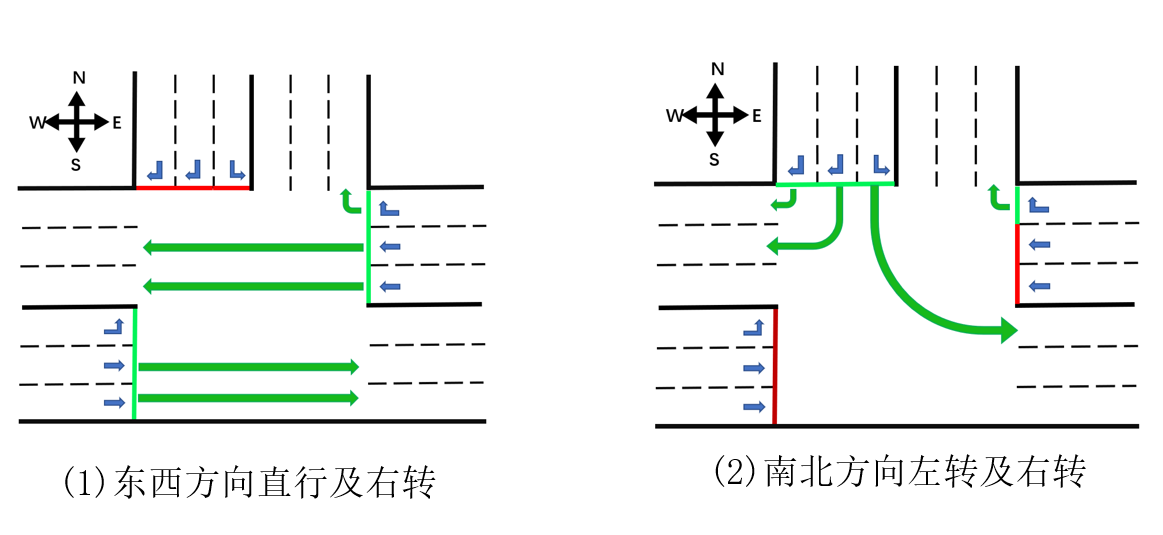
\includegraphics[width=\textwidth]{figures/T_intersection_phase.png}
	\caption{T型路口交通灯信号相位}
	\label{fig:T_intersection_phase}
\end{figure}

如图\ref{fig:baoheliulv}所示,信号相位绿灯方向的放行车流率与时间的关系。图中${t_0}$对应绿灯启亮时刻,绿灯启亮后,放行车流率不断上升,至${t_1}$时刻到达饱和车流率,随后放行车流维持饱和车流率通行,直到${t_2}$时刻绿灯周期结束,黄灯启亮,此时放行车流率不断下降,在${t_3}$时刻红灯启亮之前降低为零。

%放行车流率为单位时间内通过交叉口停车线的车辆数。

\begin{figure}[ht]
	\centering
	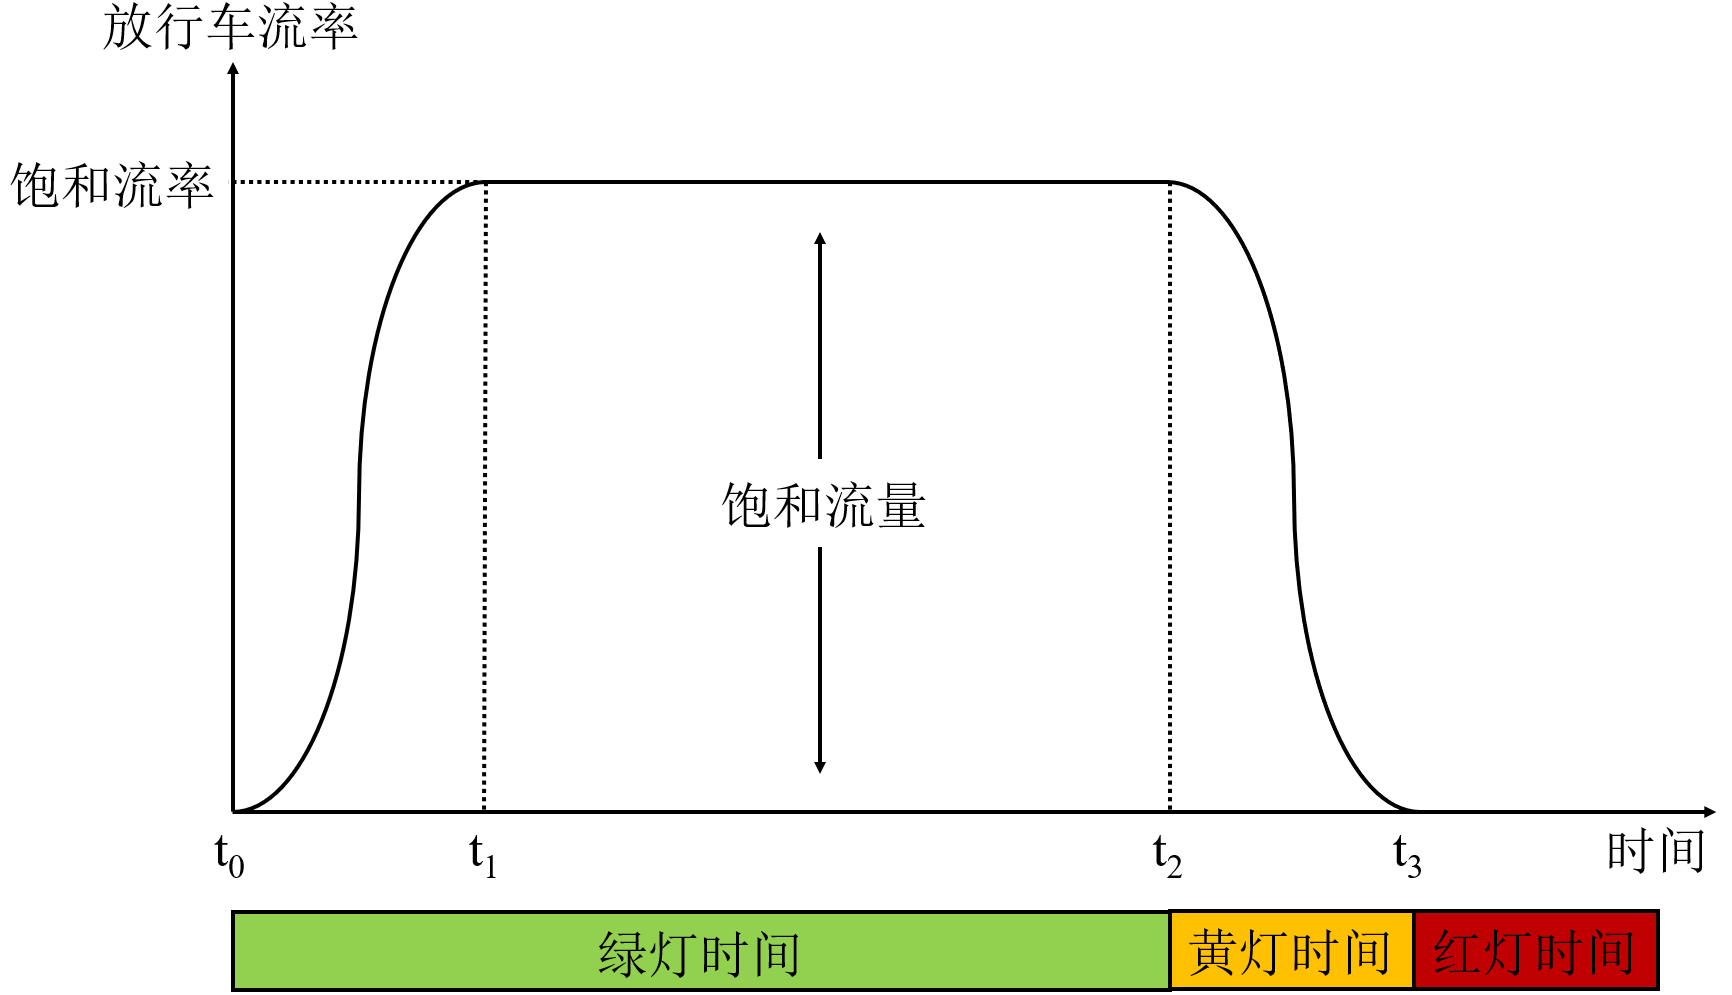
\includegraphics[width=\textwidth]{figures/baoheliulv.png}
	\caption{信号相位绿灯方向的放行车流率与时间的关系}
	\label{fig:baoheliulv}
\end{figure}


\subsection{绿波带}
%绿波带是在指定的交通线路上,当规定好路段的车速后,要求信号控制机根据路段距离,控制车流所经过的各路口绿灯起始时间,以确保车流以规定车速到达每个路口时,恰好遇到绿灯,一路顺畅通行\cite{zhaoyi,ma2019green}。如图\ref{fig:greenwave}所示。绿波带一般位于城市主干道,且交通秩序良好,没有行人和非机动车过路的路段。在绿波路段的车流车速必须维持绿波速度,才能够实现一路畅通不停车的绿波效应。

绿波带是指当车流维持在特定的速度范围内且行驶在特定的交通路线上,每当到行驶到道路交叉口时,恰好遇到的都是绿灯,保证车流一路畅通无阻\cite{zhaoyi,ma2019green}。如图\ref{fig:greenwave}所示,绿波带通常设在没有行人或非机动车横穿,且交通秩序良好的城市主干道上。只有维持在绿波速度范围内的车流,才能实现一路畅行且不停车的绿波效应。
\begin{figure}[ht]
	\centering
	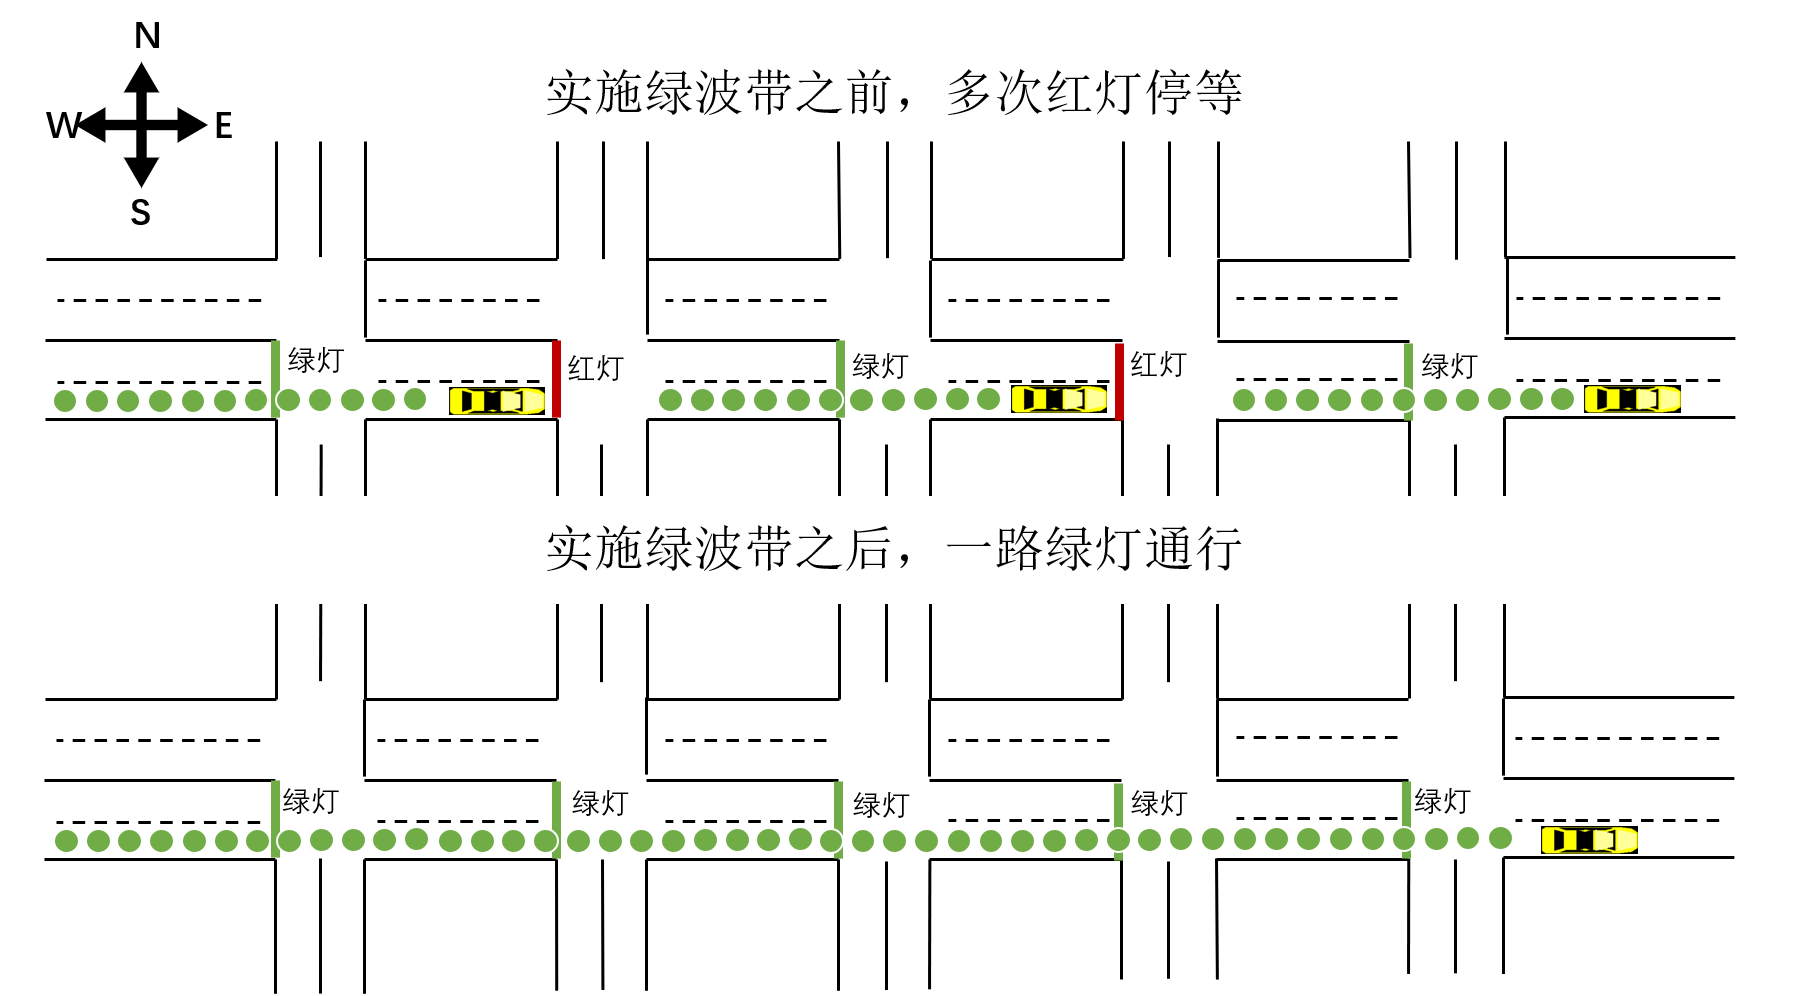
\includegraphics[width=\textwidth]{figures/greenwave.png}
	\caption{绿波带示意图}
	\label{fig:greenwave}
\end{figure}

\section{K-Means算法}
%K-Means算法\cite{K_Means_1979}用于把样本集分割成${K}$个簇,并要求簇内元素尽量密集,簇间元素尽量无关。给定一个数据集合,其中包含了${n}$个样本,每个样本都是${d}$维数据点,数据集${X=\{x_1,x_2,\ldots,x_n\}}$,其中${x_i \in R^d}$,需要生成子集的个数为${k}$,簇划分为${C=c_1, c_2, \ldots, c_k}$,每一个簇${c_i}$都有一个质心,表示簇${c_i}$均值向量,质心的值为簇内样本均值,质心定义为

%K-Means算法\cite{K_Means_1979}是无监督的聚类算法,它的算法思想是对于给定的样本集,按照样本间的距离大小,将样本集划分为${K}$个簇,让簇内的点尽量地紧密,而簇间的距离尽量的大。
K-Means算法\cite{K_Means_1979}用于把样本集分割成${K}$个簇,并要求簇内元素尽量密集,簇间元素尽量无关。给定一个数据集合,其中包含了${n}$个样本,每个样本都是${d}$维数据点,数据集${X=\{x_1,x_2,\ldots,x_n\}}$,其中${x_i \in R^d}$,需要将数据集划分为${k}$个簇,有${C=c_1, c_2, \ldots, c_k}$,每个簇都有对应的质心,表示簇${c_i}$均值向量,质心的值为簇内样本均值,质心定义为
\begin{equation}
	\mu_i=\frac{1}{\left|c_i\right|}\sum_{x\in c_i} x
\end{equation}

聚类目标是使得各簇总的平方误差${E}$最小,公式如下:

\begin{equation}
	E=\sum_{i=1}^{k}\sum_{x\in c_i}\left|\left|x-\mu_i\right|\right|_2^2
\end{equation}
%其中${\mu_i}$表示簇${C_i}$的均值向量,也可称为质心,质心的值为簇内样本均值。



K-Means算法流程如下:
\begin{enumerate}
	\item 在确定了需要生成的样本集个数${k}$后,在数据集中,随机地选择${k}$个样本作为初始质心: ${{\mu_1,\mu_2,\ldots,\mu_k}}$。%由于K-Means算法是启发式方法,${k}$个初始化的质心的位置选择对最后的聚类结果和运行时间都有很大的影响,因此需要选择合适的质心,最好这些质心不能太近。
	\item 初始化${k}$个簇,有${C_t=\phi,t=1,2,\ldots,k}$,按照样本与${k}$个质心之间的欧式距离,把他们分配给距离最近的质心所代表的簇。计算样本${x_i}$和各个质心向量${\mu_j}$的欧式距离如下式所示:
	%\item 将簇划分初始化为${C_t=\phi,t=1,2,\ldots,k}$,对于样本中的数据对象,根据他们与${k}$个质心的欧式距离,按照距离最近准则将他们分配给相应的质心所代表的簇。计算样本${x_i}(i=1,2,\ldots,n)$和各个质心向量${\mu_j (j=1,2,...k)}$的距离如下式所示:
	\begin{equation}
		d_{ij}=\left|\left|x_i-\mu_j\right|\right|_2^2
	\end{equation}
	
	\item 对于${j=1,2,...,k}$,对所有簇${C_j}$重新计算新的质心,假设每个质心都不变,那么可以转入步骤4,否则转到步骤2。
	%\item 对于${j=1,2,...,k}$,对${C_j}$中所有的样本点重新计算新的质心,如果所有的${k}$个质心向量都没有发生变化,则转到步骤4,否则转到步骤2。
	\item 聚类结束。
\end{enumerate}


%若给定足够的迭代次数,K-Means算法就能收敛,但是有可能在局部最小值点收敛。K-Means收敛局部极值的原因很可能是初始化簇类中心的距离很接近,而且算法的收敛时间也加长了,为了避免这一情况,多次运行K-Means算法,每次运行初始化不同的簇类中心。

%为了避免K-Means算法在局部最小值点收敛,应多次运算K-Means算法,并且每次初始化的质心不同。
为防止K-Means算法在局部的最小值点上收敛,将反复运算K-Means算法,并且每次初始化的质心都不同。

%\section{工具开发相关技术}

\section{二次规划}
二次规划已经被研究了几十年,自1956年二次规划算法被提出,到1986年Garcia等人\cite{Garcia_1986}利用二次规划解决动态矩阵问题,再到1995年Boggs等人\cite{Boggs_1995}对二次规划进行了梳理,到2005年Gill等人\cite{Gill_2001}提出了一种用于大规模约束优化算法,然后在2006年Nocedal等人\cite{Nocedal_2006}发表了序列二次规划,二次规划被数学家们广泛研究,且在不断地进步。

二次规划是非线性规划中的一种特殊形式,带有二次目标函以及线性约束条件,在实际生活中得到了广泛的应用,它可以用于时间调度、规模经济学、工程设计以及控制领域、设施分配、选址问题、二次分配问题以及微观经济学等很多领域中。其标准形式如下:
\begin{equation}
	\label{qp:target_sample}
	\min q(x)=\frac{1}{2}x^THx+g^Tx
\end{equation}

\begin{equation}
	s.t.
	\begin{cases}
		a_i^Tx=b_i, & i \in E \\
		h_i^Tx \leq t_j, & j \in I
	\end{cases}
	\label{equation:jump}
\end{equation}

%其中$H$是${n \times n}$的对称矩阵,需要注意的是当${H}$为正定矩阵时,用椭圆法可以在多项式时间内求解出二次规划问题,但是当${H}$不是正定矩阵时,二次规划问题就成为了一个NP难问题,即使${H}$只存在一个负特征值,二次规划问题也是NP困难的。${E,I}$分别代表对应等式约束和不等式约束的集和,${i \in E}$表示${m}$个等式约束集和,${j \in I}$表示${n}$个等式约束集和。${g}$、${x}$、${a_i(i \in E)}$和${h_j(j \in I)}$是${n}$维向量。

其中$H$是${n \times n}$的对称矩阵,需要注意的是当${H}$为正定矩阵时,可以在多项式时间内求解出二次规划问题,否则,二次规划问题就成为了一个NP难问题。${E}$代表对应等式约束集和,有${i \in E}$,${I}$代表不等式约束的集和,有${j \in I}$,假设有${m}$个等式约束集和和${n}$个不等式约束集和。${g}$、${x}$、${a_i(i \in E)}$和${h_j(j \in I)}$是${n}$维向量。

%E代表所有不等式约束的集和,I∈E代表所有m个式子的约束集和,j∈i代表n个式子的约束集和。

人们通常用内点法和积极集法求解二次规划问题。本文以内点法为例,标准形式的拉格朗日函数为

\begin{equation}
	L(x,\lambda,\mu) = \frac{1}{2}x^THx+g^Tx+\sum_{i=1}^{m}\lambda_i(a_i^T-b_i) + \sum_{j=1}^{n}\mu_j(h_j^T-t_i)
\end{equation}

%Karush-Kuhn-Tucker (KKT)条件是非线性规划(nonlinear programming)最佳解的必要条件。KKT条件将拉格朗日乘数法所处理涉及等式的约束优化问题推广至不等式。使用原始对偶内点法,向KKT条件中加入微小量${\tau}$,如下

KKT(Karush-Kuhn-Tucker)条件是非线性规划最佳解的必要条件。KKT条件使得拉格朗日乘数法可以处理不等式。应用原始对偶内点法,向KKT条件中加入微小量${\tau}$,如下所示:
\begin{equation}
	\begin{cases}
		Hx+g+\sum_{i=1}^{m}\lambda_ia_i+\sum_{j=1}^{n}\mu_jh_j=0\\
		a_i^Tx=b_i, i=1,\ldots,m \\
		h_j^Tx \leq t_j \\
		\mu_j(h_jx-t_j)=-\tau_j \\
		\mu_j \geq 0, j = 1, \ldots ,n
	\end{cases}
\end{equation}
为了验证解是否在约束空间内,在不等式方程组中引入松弛变量${s_j}$,有
\begin{equation}
	s_j=t_j-h_jx
\end{equation}
则KKT条件成为
\begin{equation}
	\begin{cases}
		Hx+g+\sum_{i=1}^{m}\lambda_ia_i+\sum_{j=1}^{n}\mu_jh_j=0\\
		a_i^Tx=b_i, i=1,\ldots,m \\
		h_j^Tx +s_j = t_j \\
		\mu_js_j=\tau_j \\
		\mu_j,s_j \geq 0, j = 1, \ldots ,n
	\end{cases}.
\end{equation}
将其写成矩阵形式为
\begin{equation}
F(x,s,\lambda,\mu)=
\begin{bmatrix}
	Hx+g+\lambda a + \mu h \\
	h^Tx+s-t \\
	a^Tx - b \\
	\mu s - \tau 
\end{bmatrix}
=0
\end{equation}
其中
\begin{equation}
	\lambda=
	\begin{bmatrix}
		\lambda_1 & 0 & \ldots & 0 \\
		0 & \lambda_2 & \ldots & 0 \\
		\vdots & \vdots & \ldots & \vdots \\
		0 & 0 & \ldots & \lambda_m
	\end{bmatrix}
\end{equation}

\begin{equation}
	a^T=
	\begin{bmatrix}
		a_1^T \\
		a_2^T \\
		\vdots \\
		a_m^T 
	\end{bmatrix}
	,
	b=
	\begin{bmatrix}
		b_1 \\
		b_2 \\
		\vdots \\
		b_m 
	\end{bmatrix}
\end{equation}

\begin{equation}
	\mu=
	\begin{bmatrix}
		\mu_1 & 0 & \ldots & 0 \\
		0 & \mu_2 & \ldots & 0 \\
		\vdots & \vdots & \ldots & \vdots \\
		0 & 0 & \ldots & \mu_n
	\end{bmatrix}
\end{equation}
\begin{equation}
	h^T=
	\begin{bmatrix}
		h_1^T \\
		h_2^T \\
		\vdots \\
		h_n^T 
	\end{bmatrix}
	,
	t=
	\begin{bmatrix}
		t_1 \\
		t_2 \\
		\vdots \\
		t_n 
	\end{bmatrix}
	,
	s=
	\begin{bmatrix}
		s_1 \\
		s_2 \\
		\vdots \\
		s_n 
	\end{bmatrix}
\end{equation}
使用牛顿法解方程组有
\begin{equation}
	\begin{bmatrix}
		H & 0 & a^T & h^T \\
		h^T & I & 0 & 0 \\
		a^T & 0 & 0 & 0 \\
		0 & \mu_k & 0 & s_k^T 
	\end{bmatrix}
	\begin{bmatrix}
		\Delta x_k \\
		\Delta s_k \\
		\Delta \lambda_k \\
		\Delta \mu_k 
	\end{bmatrix}
	= -
	\begin{bmatrix}
		Hx_k+g+\lambda_k a + \mu_k h \\
		h^Tx_k+s_k-t \\
		a^Tx_k - b \\
		\mu_ks_k - \tau_k 
	\end{bmatrix}
\end{equation}
得到$(\Delta x_k, \Delta s_k, \Delta \lambda_k, \Delta \mu_k )$后更新变量
\begin{equation}
	(x_{k+1}, s_{k+1}, \lambda_{k+1}, \mu_{k+1}) = (x_k, s_k, \lambda_k, \mu_k ) + \alpha (\Delta x_k, \Delta s_k, \Delta \lambda_k, \Delta \mu_k )
\end{equation}
同时更新
\begin{equation}
	\tau_{k+1} = - \sigma \sum_{j=1}^{n}\mu_{j,k}s_{j,k},\sigma \in [0,1]
\end{equation}
接下来进行第${k+1}$次迭代,直至得到方程的最终解。





%\section{线性规划}
%线性规划,其标准形式如下
%\begin{equation}
%	\label{qp:target_sample}
%	\min C^Tx
%\end{equation}

%\begin{equation}
%	s.t.
%	\begin{cases}
%		a_i^Tx=b_i, & i \in E, \\
%		a_i^Tx \geq b_i, & i \in I
%	\end{cases}.
%	\label{equation:jump}
%\end{equation}


\section{本章小结}
本章介绍了文章中所涉及的预备知识,首先介绍了饱和流量和饱和流率、信号相位和“绿波带”等交通工程相关知识,然后介绍了K-Means算法和二次规划以及它们的解法。
\label{ch2}



